\section{Usecase Diagram}

Her ses aktør usecase diagrammet for det realistiske system, dette erstatter aktør-kontekst diagrammet som er så simpelt
at det ikke er nødvendigt:
\begin{figure}[H]
\centering
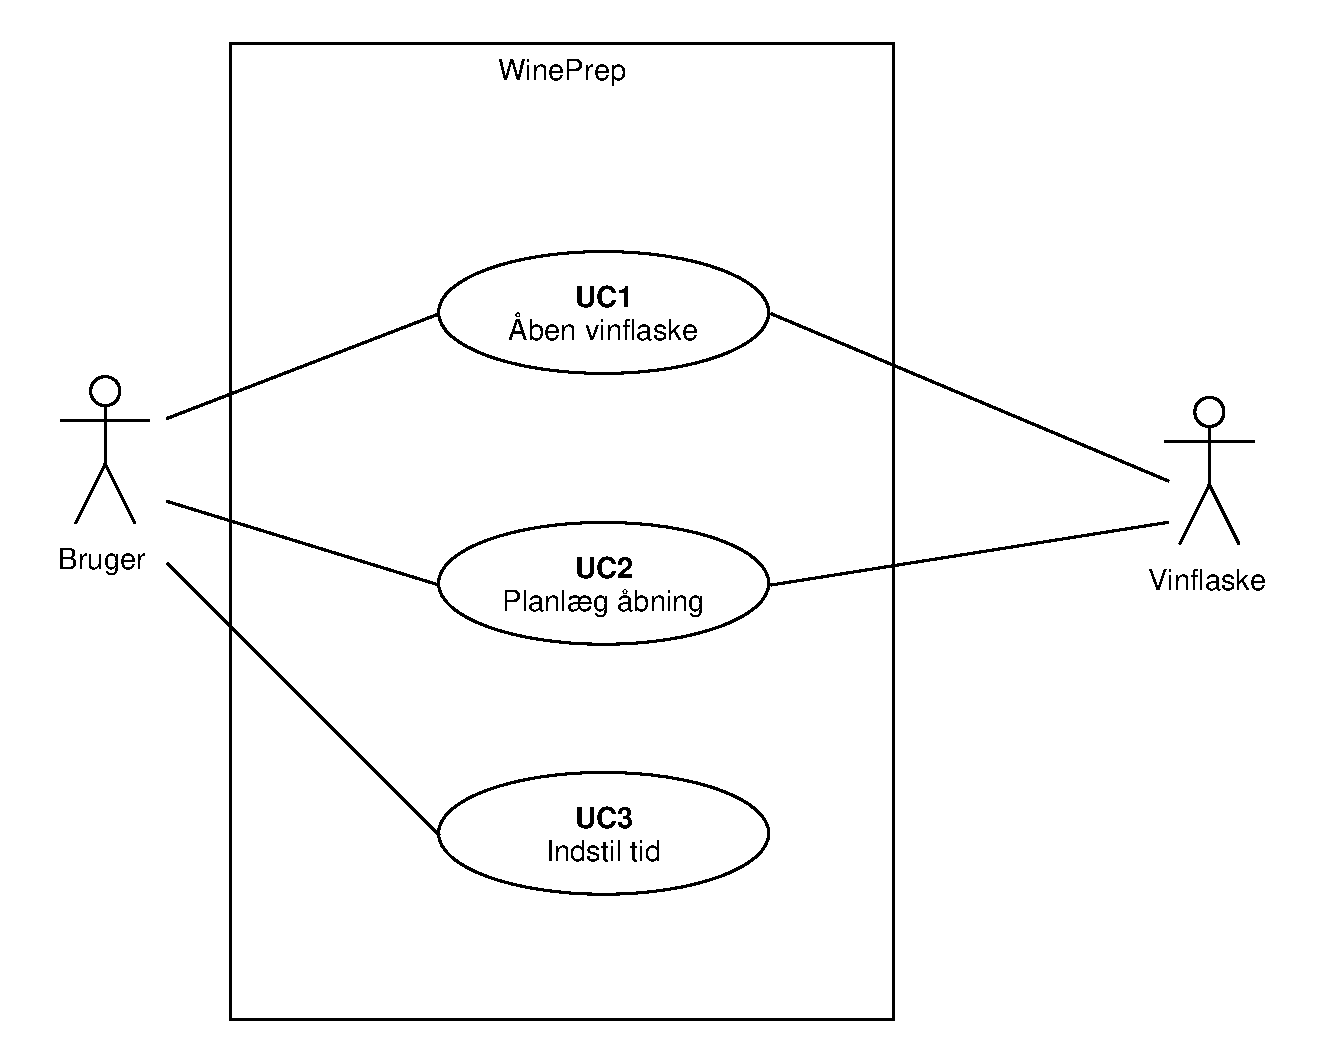
\includegraphics[scale=0.5]{usecasediagram.pdf}
\caption[Figur]{Use-case Diagram}
\end{figure}

\subsection{Aktør Beskrivelser}

\paragraph{Bruger:} Brugeren er systemets primære aktør. Brugeren er ham eller hende der betjener systemet, og har en opgave som ønskes løst af systemet.